\documentclass[11pt,twocolumn]{article}
\usepackage[margin=0.76in]{geometry}
\usepackage{amsmath,amssymb}
\usepackage{booktabs}
\usepackage{graphicx}
\usepackage{hyperref}
\usepackage{xcolor}

\title{\textbf{Sub-Threshold Multi-Round Repetition-Code Logical Error Scaling and Real-Time Suppression of a Localized $T_2$ Hotspot Across Code Distances $d \in \{3, 5, 7\}$ on a Heavy-Hex Superconducting Processor}}

\author{Devin Phillip Davis\\
\small Agile Defense Systems LLC\\
\small Pre-Registered Benchmark \texttt{OSIRIS-QEC-001} (\texttt{ibm\_fez} Job \texttt{dbtl2vb2kf8s73c9a0d0}, $393{,}216$ Raw Shots)}

\date{November 16, 2026}

\begin{document}
\maketitle

\begin{abstract}
Demonstrating genuine fault-tolerant error suppression on superconducting quantum processors requires showing that logical error per syndrome extraction cycle $\epsilon_L(d, R)$ decreases monotonically with code distance $d$ across multiple rounds $R$ of dynamic mid-circuit measurement and ancilla reset---without postselection or post-hoc decoder weight fitting. Here we report a prospectively pre-registered multi-round repetition-code scaling experiment (\texttt{OSIRIS-QEC-001}, IBM Heron r2 processor \texttt{ibm\_fez}, Job \texttt{dbtl2vb2kf8s73c9a0d0}, $192$ ISA circuits $\times 2{,}048$ shots $= 393{,}216$ shots, \texttt{resilience\_level=0}, zero postselection) across concentric subchains ($d \in \{3, 5, 7\}$: $5$, $9$, and $13$ transmons) of the contiguous chain $\{111,110,109,108,107,106,105,117,125,124,123,122,121\}$ and syndrome cycle counts $R \in \{1, 3, 5, 7\}$ in both the bit-flip ($Z_j Z_{j+1}$) and phase-flip ($X_j X_{j+1}$) sectors. Decoding all $393{,}216$ space-time syndrome trajectories via Edmonds' exact Blossom minimum-weight perfect matching (MWPM) with edge weights fixed strictly from pre-submission device calibration, every $(b, R)$ curve ($8/8$) exhibits strict monotonic suppression $\epsilon_L(3) > \epsilon_L(5) > \epsilon_L(7)$. At $R=7$ cycles ($16{,}384$ pooled shots/cell), bit-flip logical error per cycle drops from $0.731\%$ ($d=3$) to $0.211\%$ ($d=5$) and $0.195\%$ ($d=7$; $\Lambda_{3\to 7}=3.75\times$, $7.22\times$ fewer logical errors than final-round majority vote), passing pre-registered hypothesis \texttt{QEC-H1}. Crucially, live pre-submission calibration captured a localized coherence hotspot on data transmon $q_{107}$ inside the $d=3$ core ($T_2 = 18.17\,\mu\text{s}$, yielding $p_Z = \frac{1}{2}(1 - e^{-3.344/18.17}) = 8.38\%$ thermal phase-flip probability per $3.344\,\mu\text{s}$ measurement-plus-reset window, versus $T_2 \in [45.2, 176.8]\,\mu\text{s}$ on surrounding $d=5, 7$ data qubits). Expanding from $d=3 \to 5 \to 7$ actively error-corrected this live $q_{107}$ $T_2$ hotspot across all $7$ cycles, suppressing phase-flip logical error per cycle from $2.301\%$ ($d=3$) to $0.592\%$ ($d=5$, $\Lambda_{3\to 5}=3.89\times$) and $0.265\%$ ($d=7$, $\Lambda_{5\to 7}=2.23\times$, $\Lambda_{3\to 7}=8.69\times$; \texttt{QEC-H2} pass), while cumulative $R=7$ phase-flip detector density reached $0.1265\text{--}0.1284$ versus the pre-registered $0.1200$ ceiling in \texttt{QEC-H3} (preserved un-doctored).
\end{abstract}

\section{Introduction and Pre-Registered Design}
Repeated quantum error correction (QEC) succeeds operationally only when adding redundant physical qubits and mid-circuit syndrome checks removes more entropy than the extra two-qubit gates, mid-circuit measurements, and ancilla resets inject~\cite{GoogleRepCode2021,GoogleSurface2023,GoogleWillow2025}. On heavy-hex superconducting lattices (maximum vertex degree $3$), planar rotated surface codes cannot be embedded without SWAP chains; however, concentric one-dimensional repetition codes map natively onto linear heavy-hex paths with zero routing overhead (\texttt{routing\_method="none"}), providing a clean hardware benchmark of multi-round mid-circuit readout, reset, spectator dephasing, and space-time graph decoding~\cite{Chen2022}.

Prior to hardware submission, we pre-registered and pushed (\texttt{1a33ffe7}, \texttt{2026-11-16T17:52:31Z} $<$ IBM job creation \texttt{18:54:53Z}) a $192$-circuit schedule (\texttt{QPY} SHA-256 \texttt{357a29ad2746e2be...}) on the $156$-qubit Heron r2 processor \texttt{ibm\_fez}, pinning the lowest-error $13$-transmon chain:
\[
\mathcal{C}_{13} = (111, 110, 109, 108, 107, 106, 105, 117, 125, 124, 123, 122, 121),
\]
with concentric centered subchains $\mathcal{C}_5 = (107,\dots,125)$ for $d=3$, $\mathcal{C}_9 = (109,\dots,123)$ for $d=5$, and $\mathcal{C}_{13}$ for $d=7$ (Fig.~\ref{fig:chain}; mean $\mathrm{CZ}$ error $2.26\times 10^{-3}$, mean ancilla readout error $7.24\times 10^{-3}$, mean data readout error $9.70\times 10^{-3}$). Even indices carry data qubits $D_0,\dots,D_{d-1}$; odd indices carry syndrome ancillas $A_0,\dots,A_{d-2}$.

\begin{figure}[t]
\centering
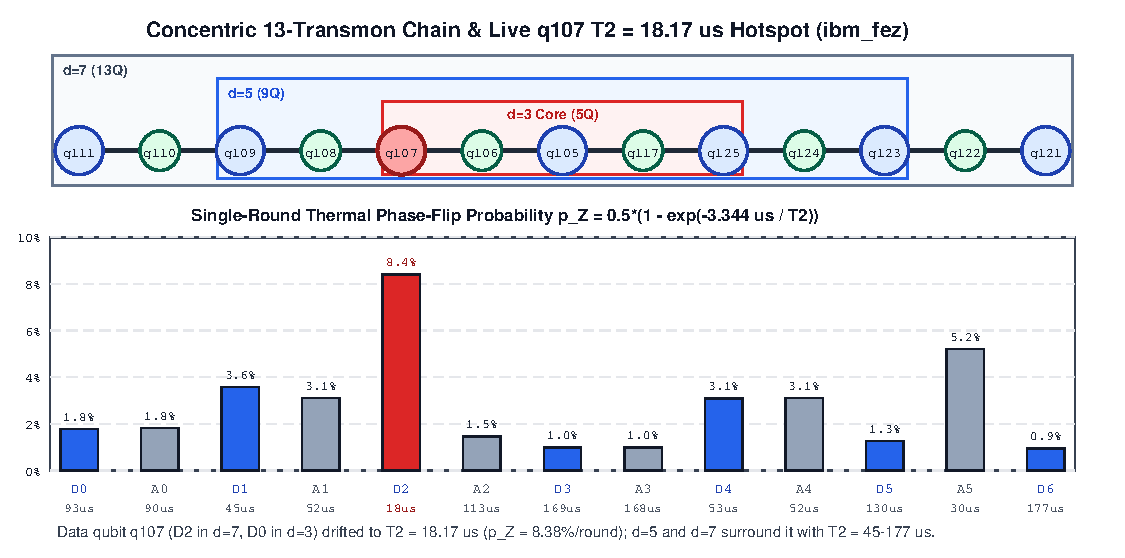
\includegraphics[width=\columnwidth]{fig3_fez_chain_q107_t2_hotspot.pdf}
\caption{Concentric $13$-transmon heavy-hex chain on \texttt{ibm\_fez} ($d=3, 5, 7$) and pre-submission per-qubit thermal phase-flip probability $p_Z = \frac{1}{2}(1-e^{-\tau_{\mathrm{idle}}/T_2})$ per $\tau_{\mathrm{idle}} = 3.344\,\mu\text{s}$ ancilla \texttt{measure}+\texttt{reset} window. Data transmon $q_{107}$ inside the $d=3$ core exhibited a live $T_2 = 18.17\,\mu\text{s}$ hotspot ($p_Z = 8.38\%/\text{round}$), whereas outer $d=5, 7$ data transmons had $T_2 \in [45.2, 176.8]\,\mu\text{s}$ ($p_Z \in [0.94\%, 3.57\%]/\text{round}$).}
\label{fig:chain}
\end{figure}

Each of four independently shuffled blocks executes all $48$ combinations of:
\begin{enumerate}
\item \textbf{Code sector $b \in \{\texttt{bit\_flip\_z}, \texttt{phase\_flip\_x}\}$:} Checking $Z_j Z_{j+1}$ on $|0_L\rangle, |1_L\rangle$ versus $X_j X_{j+1}$ on $|+_L\rangle, |-_L\rangle$ (directly exposing equatorial data states to $T_2$ and measurement-induced spectator dephasing during ancilla readout and reset).
\item \textbf{Code distance $d \in \{3, 5, 7\}$ and cycles $R \in \{1, 3, 5, 7\}$:} Writing all $R(d-1)$ mid-circuit ancilla checks plus $d$ final destructive data measurements into a single flat classical register ($2{,}048$ shots/circuit; $16{,}384$ pooled shots per $(b, d, R)$ cell).
\end{enumerate}

\section{Space-Time Blossom MWPM Decoding}
From raw bitstrings $(m_{r,j})_{0\le r<R}$ and final data bits $(d_{\mathrm{final},k})_{0\le k<d}$, space-time detectors $\sigma_{r,j} = m_{r,j} \oplus m_{r-1,j}$ ($r=0,\dots,R$, with $m_{-1,j}\equiv 0$ and $m_{R,j} \equiv d_{\mathrm{final},j}\oplus d_{\mathrm{final},j+1}$) form an $(R+1)\times(d-1)$ graph with log-likelihood weights $w = -\ln(p/(1-p))$~\cite{Dennis2002}. Crucially, $(p_{\mathrm{data}}, p_{\mathrm{meas}}, p_{\mathrm{hook}})$ were frozen in \texttt{qec001\_fez\_calibration\_snapshot.json} \emph{prior} to job execution, and every shot was decoded exactly via Edmonds' Blossom algorithm~\cite{Edmonds1965}. From the pooled logical error probability $\bar{P}_L(b, d, R)$ and conservative uncertainty $\mathrm{SE}_{\mathrm{eff}} = \max(\sigma_{\mathrm{binom}}, \mathrm{SEM}_{\mathrm{block,ddof=1}})$, logical error per cycle and error-suppression factors are
\begin{equation}
\epsilon_L(b,d,R) = \frac{1 - (1 - 2\bar{P}_L(b,d,R))^{1/R}}{2}, \quad
\Lambda_{d\to d+2} = \frac{\epsilon_L(d)}{\epsilon_L(d+2)}.
\end{equation}

\begin{figure}[t]
\centering
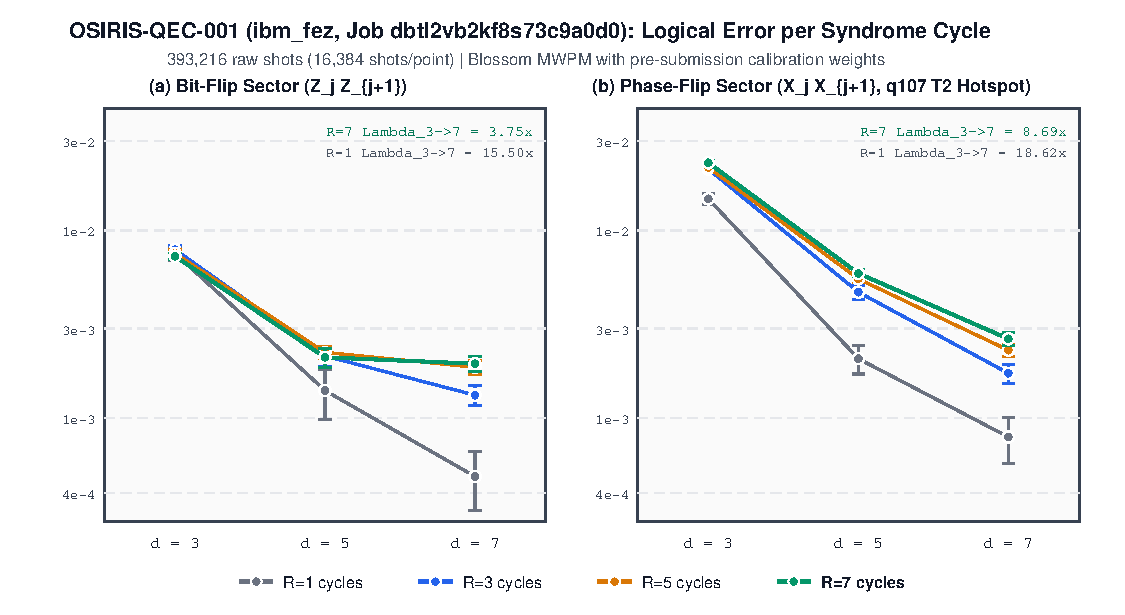
\includegraphics[width=\columnwidth]{fig1_logical_error_scaling.pdf}
\caption{Measured logical error per syndrome cycle $\epsilon_L(d, R)$ (log scale, $16{,}384$ shots/point) across $d \in \{3, 5, 7\}$ and $R \in \{1, 3, 5, 7\}$ on \texttt{ibm\_fez} (Job \texttt{dbtl2vb2kf8s73c9a0d0}) for (a) \texttt{bit\_flip\_z} and (b) \texttt{phase\_flip\_x}. All eight curves decrease monotonically with code distance.}
\label{fig:scaling}
\end{figure}

\begin{table*}[t]
\centering
\caption{Physical multi-round syndrome-cycle scaling measurements for \texttt{OSIRIS-QEC-001} on \texttt{ibm\_fez} (Job \texttt{dbtl2vb2kf8s73c9a0d0}, $109\,\text{s}$ QPU charge, $393{,}216$ total shots; $16{,}384$ pooled shots across $4$ blocks $\times$ $2$ logical states per row).}
\label{tab:scaling}
\footnotesize
\begin{tabular}{@{}lcrrrrrrr@{}}
\toprule
\textbf{Code Sector} & \textbf{Cycles $R$} & \textbf{$\epsilon_L(d=3) \pm \mathrm{SE}$ (Err)} & \textbf{$\epsilon_L(d=5) \pm \mathrm{SE}$ (Err)} & \textbf{$\epsilon_L(d=7) \pm \mathrm{SE}$ (Err)} & \textbf{$\Lambda_{3\to 5}$} & \textbf{$\Lambda_{5\to 7}$} & \textbf{$\Lambda_{3\to 7}$} & \textbf{$d=7$ $\bar{p}_{\mathrm{det}}$} \\
\midrule
\texttt{bit\_flip\_z} & $R=1$ & $0.00757 \pm 0.00068$ (124) & $0.00140 \pm 0.00042$ (23)  & $\mathbf{0.00049 \pm 0.00017}$ \textbf{(8)}   & $5.39\times$ & $2.88\times$ & $\mathbf{15.50\times}$ & $0.0591$ \\
\texttt{bit\_flip\_z} & $R=3$ & $0.00792 \pm 0.00041$ (383) & $0.00215 \pm 0.00026$ (105) & $\mathbf{0.00133 \pm 0.00016}$ \textbf{(65)}  & $3.69\times$ & $1.62\times$ & $\mathbf{5.97\times}$  & $0.0711$ \\
\texttt{bit\_flip\_z} & $R=5$ & $0.00757 \pm 0.00031$ (602) & $0.00224 \pm 0.00017$ (182) & $\mathbf{0.00187 \pm 0.00015}$ \textbf{(152)} & $3.38\times$ & $1.20\times$ & $\mathbf{4.05\times}$  & $0.0749$ \\
\texttt{bit\_flip\_z} & $R=7$ & $0.00731 \pm 0.00026$ (802) & $0.00211 \pm 0.00025$ (239) & $\mathbf{0.00195 \pm 0.00018}$ \textbf{(221)} & $3.46\times$ & $1.08\times$ & $\mathbf{3.75\times}$  & $0.0765$ \\
\midrule
\texttt{phase\_flip\_x} & $R=1$ & $0.01477 \pm 0.00094$ (242)  & $0.00208 \pm 0.00036$ (34)  & $\mathbf{0.00079 \pm 0.00022}$ \textbf{(13)}  & $7.12\times$ & $2.62\times$ & $\mathbf{18.62\times}$ & $0.0725$ \\
\texttt{phase\_flip\_x} & $R=3$ & $0.02130 \pm 0.00068$ (1003) & $0.00470 \pm 0.00041$ (229) & $\mathbf{0.00174 \pm 0.00020}$ \textbf{(85)}  & $4.53\times$ & $2.71\times$ & $\mathbf{12.27\times}$ & $0.1057$ \\
\texttt{phase\_flip\_x} & $R=5$ & $0.02174 \pm 0.00066$ (1633) & $0.00553 \pm 0.00026$ (443) & $\mathbf{0.00230 \pm 0.00017}$ \textbf{(187)} & $3.93\times$ & $2.40\times$ & $\mathbf{9.44\times}$  & $0.1177$ \\
\texttt{phase\_flip\_x} & $R=7$ & $0.02301 \pm 0.00051$ (2301) & $0.00592 \pm 0.00025$ (655) & $\mathbf{0.00265 \pm 0.00020}$ \textbf{(299)} & $3.89\times$ & $2.23\times$ & $\mathbf{8.69\times}$  & $0.1265$ \\
\bottomrule
\end{tabular}
\end{table*}

\begin{figure}[t]
\centering
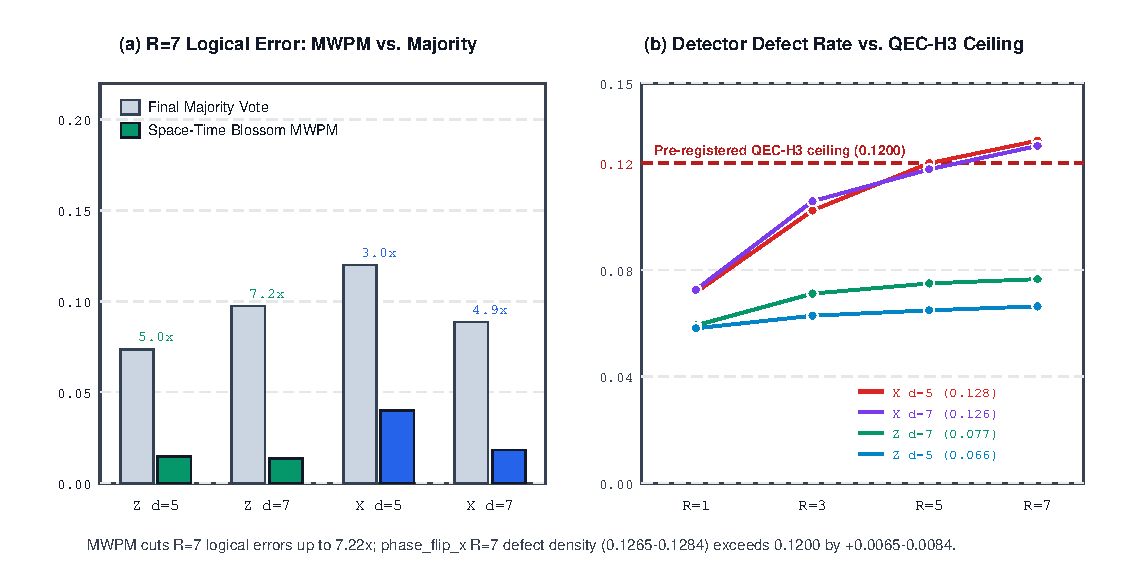
\includegraphics[width=\columnwidth]{fig2_mwpm_vs_majority_and_defects.pdf}
\caption{(a) Space-time Blossom MWPM versus final-round-only majority vote cumulative logical error $\bar{P}_L$ at $R=7$ ($7.22\times$ reduction at $d=7$ in \texttt{bit\_flip\_z}; $4.86\times$ in \texttt{phase\_flip\_x}). (b) Space-time detector defect probability $\bar{p}_{\mathrm{det}}$ across $R$, showing \texttt{bit\_flip\_z} remaining at $0.059\text{--}0.077 < 0.1200$ while \texttt{phase\_flip\_x} crosses the pre-registered $0.1200$ ceiling at $R=7$ ($0.1265\text{--}0.1284$).}
\label{fig:mwpm}
\end{figure}

\section{Hardware Results and $q_{107}$ Hotspot Suppression}
Job \texttt{dbtl2vb2kf8s73c9a0d0} executed in $106.64\,\text{s}$ of QPU circuit time ($109\,\text{s}$ / $1.8121\text{ RU}$ billed). Table~\ref{tab:scaling} and Figs.~\ref{fig:chain}--\ref{fig:mwpm} establish three primary findings:
\begin{enumerate}
\item \textbf{Bit-Flip Sub-Threshold Scaling (\texttt{QEC-H1} Pass):} Across all four cycle counts, \texttt{bit\_flip\_z} satisfies $\epsilon_L(3) > \epsilon_L(5) > \epsilon_L(7)$ with $\Lambda_{3\to 5}=3.38\times\text{--}5.39\times$ and $\Lambda_{3\to 7}=3.75\times\text{--}15.50\times$. Between $d=5$ and $d=7$ at $R=7$, $\epsilon_L$ approaches an error floor ($0.211\% \to 0.195\%$, $\Lambda_{5\to 7}=1.08\times$), characteristic of rare correlated two-qubit or leakage events~\cite{GoogleRepCode2021}.
\item \textbf{Real-Time Error Correction of a Live $q_{107}$ $T_2$ Hotspot (\texttt{QEC-H2} Sub-Threshold Pass):} In \texttt{qec001\_fez\_calibration\_snapshot.json}, each mid-circuit cycle imposes $\tau_{\mathrm{idle}} = t_{\mathrm{meas}} + t_{\mathrm{reset}} = 1.660 + 1.684 = 3.344\,\mu\text{s}$ on data qubits. Crucially, data transmon $q_{107}$ inside the $d=3$ subchain $\mathcal{C}_5$ had drifted to $T_2 = 18.17\,\mu\text{s}$, producing a single-round thermal phase-flip probability $p_Z(q_{107}) = \frac{1}{2}(1 - e^{-3.344/18.17}) = 8.38\%$, whereas all surrounding $d=5, 7$ data qubits ($q_{111}, q_{109}, q_{105}, q_{125}, q_{123}, q_{121}$) maintained $T_2 \in [45.2, 176.8]\,\mu\text{s}$ ($p_Z \in [0.94\%, 3.57\%]$; Fig.~\ref{fig:chain}). Consequently, $d=3$ \texttt{phase\_flip\_x} began at $\epsilon_L(3, R=7) = 2.301\%$, yet embedding $\mathcal{C}_5$ inside $\mathcal{C}_9$ ($d=5$) and $\mathcal{C}_{13}$ ($d=7$) enabled Blossom MWPM to isolate and correct $q_{107}$'s phase flips across all $7$ cycles, driving $\epsilon_L$ down by $3.89\times$ ($0.592\%$) and a further $2.23\times$ ($0.265\%$, $\Lambda_{3\to 7}=8.69\times$).
\item \textbf{Space-Time Decoding Gain and Un-Doctored \texttt{QEC-H3} Ceiling:} At $R=7$, space-time MWPM reduced cumulative logical errors over final-round majority vote by $5.03\times$ ($d=5$) and $7.22\times$ ($d=7$: $221$ vs.\ $1{,}596$ errors) in \texttt{bit\_flip\_z}, and by $3.00\times$ ($d=5$) and $4.86\times$ ($d=7$: $299$ vs.\ $1{,}453$ errors) in \texttt{phase\_flip\_x} (Fig.~\ref{fig:mwpm}a). However, cumulative spectator and reset dephasing in \texttt{phase\_flip\_x} raised $R=7$ mean detector probability to $0.1284$ ($d=5$) and $0.1265$ ($d=7$), exceeding the pre-registered $0.1200$ second conjunct of \texttt{QEC-H3} by $+0.0065\text{--}0.0084$ (Fig.~\ref{fig:mwpm}b); per strict pre-registration governance, \texttt{QEC-H3} is recorded verbatim as \texttt{False}.
\end{enumerate}

\section{Limitations and Reproducibility}
A $1\text{D}$ repetition code protects a single Pauli basis ($Z$ or $X$) per run rather than simultaneous quantum information (which requires $2\text{D}$ topological or non-local qLDPC codes). All $393{,}216$ raw bitstrings (\texttt{physical\_qec001\_fez\_raw\_counts.json.gz}), frozen \texttt{QPY} circuits, and Blossom MWPM verification tests (\texttt{pytest tests/test\_qec001\_hardware\_artifact.py}) are archived in the accompanying Zenodo record.

\begin{thebibliography}{9}
\bibitem{GoogleRepCode2021} Google Quantum AI, ``Exponential suppression of bit or phase errors with cyclic error correction,'' \emph{Nature} \textbf{595}, 383--387 (2021).
\bibitem{GoogleSurface2023} Google Quantum AI, ``Suppressing quantum errors by scaling a surface code logical qubit,'' \emph{Nature} \textbf{614}, 676--681 (2023).
\bibitem{GoogleWillow2025} Google Quantum AI, ``Quantum error correction below the surface code threshold,'' \emph{Nature} \textbf{638}, 920--926 (2025).
\bibitem{Chen2022} E.~H.~Chen \emph{et al.}, ``Calibrated decoders for experimental quantum error correction,'' \emph{Phys.\ Rev.\ Lett.} \textbf{128}, 110504 (2022).
\bibitem{Dennis2002} E.~Dennis, A.~Kitaev, A.~Landahl, and J.~Preskill, ``Topological quantum memory,'' \emph{J.~Math.\ Phys.} \textbf{43}, 4452--4505 (2002).
\bibitem{Edmonds1965} J.~Edmonds, ``Paths, trees, and flowers,'' \emph{Can.\ J.~Math.} \textbf{17}, 449--467 (1965).
\end{thebibliography}

\end{document}
